\documentclass[12pt]{article}
\usepackage[T1]{fontenc}
\usepackage[polish]{babel}
\usepackage[utf8]{inputenc}
\usepackage{geometry}
\usepackage{amsmath}
\usepackage{graphicx}
\graphicspath{ {./images/} }
\geometry{a4paper, margin=2cm}
\begin{document}
\textbf{Dominik Seredyn, 320732, grupa 5, projekt 1, zadanie 33}
\section{Wstęp}
Zadanie dotyczyło obliczenia całki podwójnej z podanej funkcji f na prostokącie
$D=<a,b>\times<c,d>$. Należało wykorzystać złożoną kwadraturę Newtona 3/8 ze względu na zmienną x oraz złożoną kwadraturę trapezów ze względu na zmienną y. Po ich zaimplementowaniu przeprowadziłem szereg testów, które sprawdzały, czy funkcja działa zgodnie ze specyfikacją, czy realizuje zadanie oraz własności numeryczne samej metody (np. błąd dla różnych grup funkcji).
\section{Opis metody}
Metoda polega na zastosowaniu złożonej kwadratury Newtona 3/8 do obliczenia całki wewnętrznej ze względu na zmienną $x$ na przedziale $<a,b>$. W tym celu, dzielimy go na $n$ podprzedziałów, wówczas $H_{x}=\frac{b-a}{n}$, a metoda jest dana wzorem:
\[
\sum_{k=1}^{n} (\frac{H_{x}}{8}f(x_{k-1})+\frac{3H_{x}}{8}f(\frac{2x_{k-1}+x_{k}}{3})+\frac{3H_{x}}{8}f(\frac{x_{k-1}+2x_{k}}{3})+\frac{H_{x}}{8}f(x_{k})).
\]
Zatem wektor jej współczynników to $N=\frac{H_{x}}{8}\begin{bmatrix}1 & 3 & 3 & 2 &  ... & 3 & 3 & 1\end{bmatrix}$. \\
Następnie stosujemy złożoną kwadraturę trapezów do obliczenia całki ze względu na zmienną $y$ na przedziale $<c,d>$  z otrzymanej funkcji jednej zmiennej. W tym celu, dzielimy go na $m$ podprzedziałów, wówczas $H_{y}=\frac{d-c}{m}$, a metoda jest dana wzorem:
\[
\sum_{k=1}^{m} (\frac{H_{y}}{2}f(y_{k-1})+\frac{H_{y}}{2}f(y_{k})).
\]
Zatem wektor jej współczynników to $T=\frac{H_{y}}{2}\begin{bmatrix}1 & 2 & ... & 2 & 1\end{bmatrix}$. \\
W celu zrealizowania tych obliczeń tworzymy macierz C współczynników potrzebnych do obliczenia całki podwójnej. W tym przypadku:
\[
C=
T^T*N=
\frac{H_{x}H_{y}}{16}
\begin{bmatrix}
1 & 3 & 3 & 2 &  ... & 3 & 3 & 2 & 1 \\
2 & 6 & 6 & 4 &  ... & 6 & 6 & 4 & 2 \\
. & . & . & . &  ... & . & . & . & . \\
2 & 6 & 6 & 4 &  ... & 6 & 6 & 4 & 2 \\
1 & 3 & 3 & 2 &  ... & 3 & 3 & 2 & 1 \\
\end{bmatrix}
\]
Następnie tworzymy macierz W wartości funkcji w węzłach, $W(i,j)=f(x_{i},y_{j})$.
Wynikowa całka jest sumą elementów macierzy S powstałej poprzez pomnożenie macierzy C i W element po elemencie ($S(i,j)=C(i,j)*W(i,j)$). \\
Błąd złożonej metody Newtona 3/8 wyraża się wzorem $E(f)=-\frac{3}{80}H_{x}^4f^{(4)}(\xi_{3})$, $\xi_{3}\in (c,d)$. Jest to zatem metoda 4 rzędu, ze względu na czwartą pochodną we wzorze należy się spodziewać, że dla wielomianów, w których $x$ występuje co najwyżej w 3 potędze błąd będzie wynosił 0, czyli metoda będzie dokładna.
\\
Błąd metody trapezów wyraża się wzorem $E(f)=-\frac{1}{12}H_{y}^2f^{('')}(\xi_{3})$, $\xi_{3}\in (c,d)$. Jest to zatem metoda 2 rzędu, ze względu na drugą pochodną we wzorze należy się spodziewać, że dla wielomianów, w których $y$ występuje co najwyżej w 1 potędze błąd będzie wynosił 0, czyli metoda będzie dokładna.
\\
Ponadto, łatwo zauważyć, że aby uzyskać podobny błąd dla obu zmiennych należy użyć $m=n^2$.
\section{Opis testów}
\subsection{Podział testów:}
\begin{itemize}
\item{testy poprawności - test1, test2 i test3}
\item{testy sprawdzające, czy została zaimplementowana dobra metoda - test3 i test4}
\item{testy numeryczne metody- test4, test5, test6 i test7}
\end{itemize}
\subsection{Szczegółowy opis testów:}
\begin{itemize}
\item{test1 - sprawdzenie poprawości implementacji metody poprzez przetestowanie jej działania dla prostych wielomianów}
\item{test2 - test wydajności implementacji poprzez jej wykonanie dla dużej ilości podprzedziałów i wypisanie czasu działania, przy okazji sprawdza, czy program działa wtedy poprawnie}
\item{test3 - eksperymentalne sprawdzenie rzędu metody poprzez wykonywanie jej dla wielomianów coraz wyższego stopnia}
\item{test4 - eksperymentalne wyznaczenie rzędu błędu metody poprzez wykonywanie jej dla coraz większej liczby podprzedziałów}
\item{test5 - próba naszkicowania przybliżonego wykresu O(n) dla zaimplementowanej metody}
\item{test6 - test numeryczny, sprawdzający, jak zmienia się błąd metody dla różnych typów funkcji podcałkowych przy tej samej liczbie podprzedziałów}
\item{test7 - test numeryczny, pokazujący na wykresie, jak zmienia się błąd metody w zależności od miary D przy stałej liczbie podprzedziałów}
\end{itemize}
\subsection{Otrzymane wyniki:}
Z testów wynika, że zaimplementowana funkcja działa zgodnie ze specyfikacją oraz realizuje zadaną metodę. Ponadto, eksperymenty numeryczne pokazują, że metoda daje dużo dokładniejsze wyniki dla funkcji, które zmieniają się powoli np. funkcje trygonometryczne, funkcje logarytmiczne. W ich przypadku wystarczy użyć $n=10$ i $m=100$, aby uzyskać dobre przybliżenie wyniku. W przypadku funkcji wykładniczej, która zmienia się bardzo szybko, podobny błąd uzyskujemy dopiero dla $n=100$ i $m=10 000$. \\
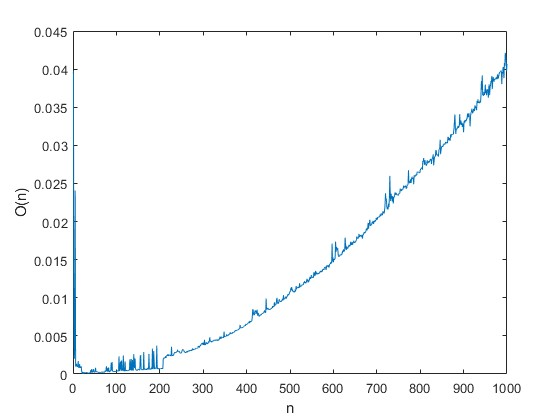
\includegraphics[scale=0.4]{test4}        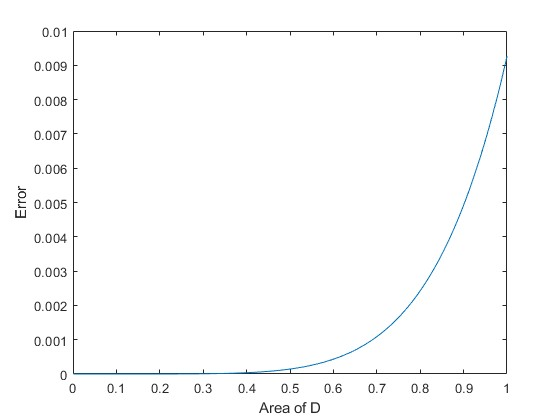
\includegraphics[scale=0.4]{test7} \\
Przybliżona złożoność obliczeniowa \quad \quad \quad \quad \quad \quad  Wpływ miary D na błąd metody \\ zaimplementowanej metody

\end{document}
